% GENERATED BY sshrc_figures.py - edit that file, not this one.
% The document that inputs this file supplies the float, the caption and the label.
% Stream A. Committees, left to right within each year: Economics, Business (14A, 14B, 14C), Multidisciplinary humanities, Multidisciplinary social sciences (23, 23A, 23B).
\definecolor{sshrcA}{HTML}{2A78D6}
\definecolor{sshrcB}{HTML}{EB6834}
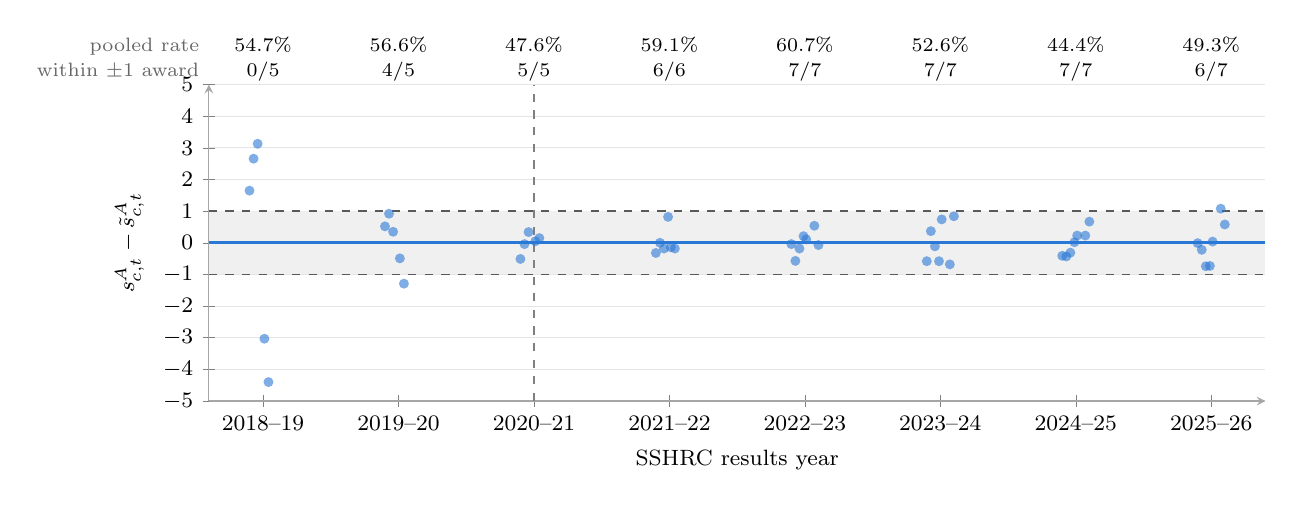
\begin{tikzpicture}
\begin{axis}[
  width=15cm, height=5.6cm,
  xmin=2017.6, xmax=2025.4, ymin=-5, ymax=5,
  xtick={2018,2019,2020,2021,2022,2023,2024,2025}, xticklabels={2018--19,2019--20,2020--21,2021--22,2022--23,2023--24,2024--25,2025--26},
  axis x line=bottom, axis y line=left, axis line style={gray!70},
  ymajorgrids, grid style={gray!20},
  tick label style={font=\footnotesize}, label style={font=\footnotesize},
  xlabel={SSHRC results year}, ylabel={$s^{A}_{c,t}-\tilde{s}^{A}_{c,t}$}, ylabel style={align=center},
  clip=false,
  ytick distance=1,
]
\fill[gray!12] (axis cs:2017.6,-1) rectangle (axis cs:2025.4,1);
\draw[gray, dashed, line width=0.7pt] (axis cs:2020,-5) -- (axis cs:2020,5);
\addplot[color=sshrcA, line width=1.2pt, forget plot, domain=2017.6:2025.4, samples=2] {0};
\addplot[gray!70!black, line width=0.7pt, dashed, forget plot, domain=2017.6:2025.4, samples=2] {-1};
\addplot[gray!70!black, line width=0.7pt, dashed, forget plot, domain=2017.6:2025.4, samples=2] {1};
\addplot[only marks, mark=*, mark size=1.8pt, color=sshrcA,
  mark options={fill opacity=0.6, draw opacity=0}]
  coordinates {(2017.93,2.66) (2017.96,3.13) (2017.90,1.65) (2018.01,-3.03) (2018.04,-4.40) (2018.93,0.92) (2018.96,0.35) (2018.90,0.52) (2019.01,-0.49) (2019.04,-1.29) (2019.90,-0.51) (2019.93,-0.04) (2019.96,0.34) (2020.01,0.05) (2020.04,0.15) (2020.90,-0.32) (2020.93,0.00) (2020.96,-0.18) (2020.99,0.82) (2021.01,-0.14) (2021.04,-0.18) (2021.90,-0.04) (2021.93,-0.57) (2021.96,-0.18) (2021.99,0.21) (2022.01,0.11) (2022.07,0.54) (2022.10,-0.07) (2022.90,-0.58) (2022.93,0.37) (2022.96,-0.11) (2022.99,-0.58) (2023.01,0.74) (2023.07,-0.68) (2023.10,0.84) (2023.90,-0.41) (2023.93,-0.43) (2023.96,-0.31) (2023.99,0.02) (2024.01,0.23) (2024.07,0.23) (2024.10,0.67) (2024.90,-0.01) (2024.93,-0.22) (2024.96,-0.74) (2024.99,-0.73) (2025.01,0.04) (2025.07,1.08) (2025.10,0.58)};
\node[font=\scriptsize, anchor=base east, text=gray!80!black] at ([yshift=12pt]axis cs:2017.6,5) {pooled rate};
\node[font=\scriptsize, anchor=base] at ([yshift=12pt]axis cs:2018,5) {54.7\%};
\node[font=\scriptsize, anchor=base] at ([yshift=12pt]axis cs:2019,5) {56.6\%};
\node[font=\scriptsize, anchor=base] at ([yshift=12pt]axis cs:2020,5) {47.6\%};
\node[font=\scriptsize, anchor=base] at ([yshift=12pt]axis cs:2021,5) {59.1\%};
\node[font=\scriptsize, anchor=base] at ([yshift=12pt]axis cs:2022,5) {60.7\%};
\node[font=\scriptsize, anchor=base] at ([yshift=12pt]axis cs:2023,5) {52.6\%};
\node[font=\scriptsize, anchor=base] at ([yshift=12pt]axis cs:2024,5) {44.4\%};
\node[font=\scriptsize, anchor=base] at ([yshift=12pt]axis cs:2025,5) {49.3\%};
\node[font=\scriptsize, anchor=base east, text=gray!80!black] at ([yshift=3pt]axis cs:2017.6,5) {within $\pm1$ award};
\node[font=\scriptsize, anchor=base] at ([yshift=3pt]axis cs:2018,5) {0/5};
\node[font=\scriptsize, anchor=base] at ([yshift=3pt]axis cs:2019,5) {4/5};
\node[font=\scriptsize, anchor=base] at ([yshift=3pt]axis cs:2020,5) {5/5};
\node[font=\scriptsize, anchor=base] at ([yshift=3pt]axis cs:2021,5) {6/6};
\node[font=\scriptsize, anchor=base] at ([yshift=3pt]axis cs:2022,5) {7/7};
\node[font=\scriptsize, anchor=base] at ([yshift=3pt]axis cs:2023,5) {7/7};
\node[font=\scriptsize, anchor=base] at ([yshift=3pt]axis cs:2024,5) {7/7};
\node[font=\scriptsize, anchor=base] at ([yshift=3pt]axis cs:2025,5) {6/7};
\end{axis}
\end{tikzpicture}
